\section{Método de volumes finitos para equações elípticas} % Seções são adicionadas para organizar sua apresentação em blocos discretos, todas as seções e subseções são automaticamente exibidas no índice como uma visão geral da apresentação, mas NÃO são exibidas como slides separados.

%----------------------------------------------------------------------------------------

\begin{frame}{Método de volumes finitos para equações elípticas}
  O objetivo desta seção é aproximar numericamente a solução do sistema \eqref{eq246} com simplificações:
  \begin{equation}\label{escoamento_base}
  \left\{
    \begin{aligned}
      - \nabla \cdot (K \nabla p) &= q && \text{em } \Omega \\
      p &= p_b && \text{em } \partial\Omega_p \\
      (-K \nabla p) \cdot n &= u_b && \text{em } \partial\Omega_u
    \end{aligned}
  \right.,
  \end{equation}
  no caso de um escoamento monofásico, com as hipóteses de ser incompressível, isotérmico e sem efeito gravitacional, de viscosidade $\mu$ e massa específica $\rho$ constantes e unitárias.

  Ademais, tem pressão relacionada a velocidade de Darcy
  \begin{equation}
    u = - K \nabla p.
  \end{equation}
\end{frame}

%----------------------------------------------------------------------------------------

\begin{frame}{Método de volumes finitos para equações elípticas}
  Para obter uma discretização de volumes finitos, integra-se a primeira equação de \eqref{escoamento_base} sobre um volume de controle genérico $V_k$:
  \begin{equation}
    - \int_{V_k}\nabla \cdot (K \nabla p)\ dx = \int_{V_k} q\ dx
  \end{equation}
  e com o teorema da divergência,
  \begin{equation}\label{eq:eq44}
    - \int_{\partial V_k}(K \nabla p) \cdot n_k\ ds = \int_{V_k} q\ dx,
  \end{equation}
  em que $n_k$ é o vetor normal à $V_k$.
\end{frame}

%----------------------------------------------------------------------------------------

\begin{frame}{Caso unidimensional}
  Considerando um domínio unidimensional $\Omega = [a,b]$ onde a primeira equação de \eqref{escoamento_base} é escrita como
  \begin{equation}\label{eq45}
    \frac{d}{dx}\left(K\frac{dp}{dx}\right) = q.
  \end{equation}
  Na discretização por volumes finitos, têm-se uma partição do domínio em $N$ intervalos $V_i = [x_{i-1/2},x_{i+1/2}]$ e integrando a equação em qualquer $V_i$,
  \begin{equation}\label{eq_1DfullequationVF}
    -\int_{x_{i-1/2}}^{x_{i+1/2}}q\ dx = \int_{x_{i-1/2}}^{x_{i+1/2}}\frac{d}{dx}\left(K\frac{dp}{dx}\right)\ dx = \left.K\frac{dp}{dx}\right|_{x_{i+1/2}} - \left.K\frac{dp}{dx}\right|_{x_{i-1/2}}.
  \end{equation}
  Dada permeabilidade absoluta é constante em cada volume de controle, têm-se uma situação como abaixo
  \begin{figure}[H]
  \centering
  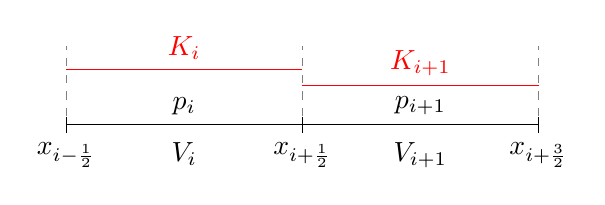
\begin{tikzpicture}[scale=1]
      % Eixo x
      \draw[black] (-1,0) -- (5,0);
      
      % Linhas da malha
      \foreach \x in {-1,2,5} {
        \draw[dashed, gray] (\x,-0.1) -- (\x,1);
        \draw[black] (\x,-0.1) -- (\x,0.1);
      }
      
      % x
      \node[below] at (-1,-0.1) {$x_{i-\frac{1}{2}}$};
      \node[below] at (2, -0.1) {$x_{i+\frac{1}{2}}$};
      \node[below] at (5, -0.1) {$x_{i+\frac{3}{2}}$};

      % V
      \node[below] at ( .5,-0.1) {$V_{i}$};
      \node[below] at (3.5,-0.1) {$V_{i+1}$};

      % K
      \draw[red] (-1,.7) -- (2,.7);
      \draw[red] (2,.5) -- (5,.5);
      \node[red, above] at ( .5,.7) {$K_{i}$};
      \node[red, above] at (3.5,.5) {$K_{i+1}$};

      % pressaum
      \node[above] at ( .5, 0) {$p_{i}$};
      \node[above] at (3.5, 0) {$p_{i+1}$};
  \end{tikzpicture}
  \caption{Esquema de volumes finitos unidimensional.}
  \label{fig:esq_VF1D}
  \end{figure}
\end{frame}

%----------------------------------------------------------------------------------------

\begin{frame}{Caso unidimensional}
  No método de volumes finitos, a pressão é interpretada como sendo uma aproximação para a média da solução exata no volume de controle $V_i$, 
  \[
    p_i \simeq \frac{1}{|V_i|}\int_{V_i}p(x)\ dx.
  \]
  Supondo a existência de um valor intermediário $p_{i+1/2}$ em $x_{i+1/2}$, discretiza-se o fluxo em cada lado de $x_{i+1/2}$ para encontrar um valor de $p_{i+1/2}$ que preserve o fluxo entre os volumes de controle. Portanto,
  \[
    \lim_{x \rightarrow x_{i+1/2}^{-}}K\frac{dp}{dx} \simeq K_i\frac{p_{i+1/2} - p_i}{\Delta x_i/2}
    \quad \text{e} \quad
    \lim_{x \rightarrow x_{i+1/2}^{+}}K\frac{dp}{dx} \simeq K_{i+1}\frac{p_{i+1} - p_{i+1/2}}{\Delta x_{i+1}/2}.
  \]
  Impondo a continuidade de fluxo nas interfaces,
  \[
    \lim_{x \rightarrow x_{i+1/2}^{-}}K\frac{dp}{dx} = \lim_{x \rightarrow x_{i+1/2}^{+}}K\frac{dp}{dx},
  \]
  ou seja, os fluxos discretos devem satisfazer 
  \[
    K_i\frac{p_{i+1/2} - p_i}{\Delta x_i} = K_{i+1}\frac{p_{i+1} - p_{i+1/2}}{\Delta x_{i+1}}.
  \]
\end{frame}

%----------------------------------------------------------------------------------------

\begin{frame}{Caso unidimensional}
  Desenvolvendo a equação e considerando que $\Delta x_{i+1} = \Delta x_{i} = \Delta x$,
  \begin{equation}
    \left.K\frac{dp}{dx}\right|_{x_{i+1/2}} = \frac{2K_iK_{i+1}}{K_i + K_{i+1}}\left(\frac{p_{i+1} - p_{i}}{\Delta x}\right).
  \end{equation}
  Logo, o coeficiente que torna o método \textbf{conservativo} é a média harmônica entre $K_i$ e $K_{i+1}$ e que define o valor adequado de $K$ em $x_{i+1/2}$.

  Voltando para \eqref{eq_1DfullequationVF}, resta aproximar a integral do lado esquerdo em
  \[
    \int_{x_{i-1/2}}^{x_{i+1/2}}q\ dx = \Delta x q_i,
  \]
  onde $q_i$ é o valor médio do termo fonte em $V_i$ e, portanto, constante por partes. Tomando
  \begin{equation}
    K_{i+1/2} = \frac{2K_iK_{i+1}}{K_i + K_{i+1}},
  \end{equation}
  a equação \eqref{eq_1DfullequationVF} em cada volume $V_i$ é dada por
  \begin{equation}\label{esquemaNum420}
    -\frac{1}{\Delta x^2}\left(K_{i+1/2}(p_{i+1} - p_{i}) - K_{i-1/2}(p_{i} - p_{i-1})\right) = q_i.
  \end{equation}
\end{frame}

%----------------------------------------------------------------------------------------

\begin{frame}{Caso unidimensional: Implementação}
  Para implementar o método de volumes finitos, considera-se o esquema numérico \eqref{esquemaNum420} escrito em forma matricial, com $N$ células
  \begin{equation}\label{forma_matricial_1d}
    Aw = d,
  \end{equation}
  com $w$ e $d$ representando os vetores de valores aproximados para a pressão e os de injeção $q$. Por fim, $A$ é uma matriz tridiagonal definida por
  \begin{equation}
    (Aw)_i = \frac{1}{\Delta x^2}\left(-K_{i-\frac{1}{2}}p_{i-1}+\left(K_{i-\frac{1}{2}}+K_{i+\frac{1}{2}}\right)p_i-K_{i+\frac{1}{2}}p_{i+1}\right),
  \end{equation}
  para $i = 2,...,N-1$. Supondo o contexto de uma malha centrada em células, as linhas $i=1$ e $i=N$ da matriz são usadas para impor condições de contornos que, neste seguinte exemplo explicativo, são de Neumann à esquerda e de Dirichlet à direita.
\end{frame}

%----------------------------------------------------------------------------------------

\begin{frame}{Caso unidimensional: Implementação}
  \textbf{Contorno de Neumann}, quando $i = 1$, a condição de contorno à esquerda estaria na célula $x_{i-1/2} = x_{1/2}$. Então, com
  \[
    - \left.K\frac{dp}{dx}\right|_{x_{\frac{1}{2}}} = u_b,
  \]
  para a primeira equação do sistema \eqref{forma_matricial_1d},
  \[
  \begin{aligned}
    - \left(\left.K\frac{dp}{dx}\right|_{x_{\frac{3}{2}}} - \left.K\frac{dp}{dx}\right|_{x_{\frac{1}{2}}}\right) &= \Delta x q_1 \\
    \frac{2K_1K_{2}}{K_1 + K_{2}}\left(\frac{p_2 - p_1}{\Delta x}\right) &= \Delta xq_1 + u_b
  \end{aligned}
  \]
  ou ainda:
  \[
    \frac{1}{\Delta x^2}\left(-K_{\frac{3}{2}}(p_2-p_1)\right) = q_1 + \frac{u_b}{\Delta x}
  \]
  e poderia ser feito na extremidade oposta de forma similar, caso necessário.
\end{frame}

%----------------------------------------------------------------------------------------

\begin{frame}{Caso unidimensional: Implementação}
  \textbf{Contorno de Dirichlet}, quando $i = N$, a face $x_{N+1/2}$, tem pressão imposta
  \[
    \left.p\right|_{x_{N+1/2}} = p_b
  \]
  e então a última equação do sistema \eqref{forma_matricial_1d} seria, portanto,
  \begin{equation}\label{eq428}
    - \left(\left.K\frac{dp}{dx}\right|_{x_{N+\frac{1}{2}}} - \left.K\frac{dp}{dx}\right|_{x_{N-\frac{1}{2}}}\right) = \Delta x q_N.
  \end{equation}
  Para este exemplo de contorno Dirichlet, será usada uma discretização com meio volume de controle:
  \[
    \left.K\frac{dp}{dx}\right|_{x_{N+\frac{1}{2}}} = K_N\left(\frac{p_b - p_N}{\Delta x/2}\right) = 2K_N\left(\frac{p_b - p_N}{\Delta x}\right)
  \]
  Dessa forma, em \eqref{eq428}:
  \[
    \frac{1}{\Delta x^2}\left(2K_{N}p_N + K_{N-\frac{1}{2}}(p_N-p_{N-1})\right) = q_1 + \frac{2K_{N}p_b}{\Delta x^2}
  \]
  e poderia ser feito na extremidade oposta de forma similar, caso necessário.
\end{frame}

%----------------------------------------------------------------------------------------

\begin{frame}{Caso unidimensional: Implementação}
  Portanto, a matriz $A$ do sistema, considerando as duas condições de contorno (de Neumann pela esquerda e de Dirichlet pela direita) é dada por
  \[
    A = \frac{1}{\Delta x^2}
    \begin{bmatrix}
      K_{\frac{3}{2}}  & -K_{\frac{3}{2}} & & & &  \\
      -K_{\frac{3}{2}} & \left(K_{\frac{3}{2}} + K_{\frac{5}{2}}\right) & -K_{\frac{5}{2}}   & & & \\
      & \ddots & \ddots & \ddots & & \\
      & & -K_{N-\frac{3}{2}} & \left(K_{N-\frac{3}{2}} + K_{N-\frac{1}{2}}\right) & -K_{N-\frac{1}{2}} \\
      & & & -K_{N-\frac{1}{2}} & \left(K_{N-\frac{1}{2}} + 2 K_{N}\right)
    \end{bmatrix}
  \]
  e
  \[
    d^t = 
    \left(
      q_1 + \frac{u_b}{\Delta x},\ q_2,\ \cdots,\ q_{N-1},\ q_N + \frac{2K_{N}p_b}{\Delta x^2}
    \right).
  \]
\end{frame}

%----------------------------------------------------------------------------------------

\begin{frame}{Caso unidimensional: Implementação}
  Foram realizados testes com os três algoritmos de fatoração: $\mathbf{LDL^T}$, de \textbf{Crout} e de \textbf{Cholesky}. Pode-se ver que o método $\mathbf{LDL^T}$ performou melhor que a fatoração de Crout (pensando no problema do exemplo desta seção).
  \begin{table}[h]
    \centering
    \begin{tabular}{|c|c|c|c|}
      \hline
      \textbf{Subintervalos} & $\mathbf{LDL^t}$ & \textbf{Crout} & \textbf{Cholesky} \\
      \hline\hline
      $10^2$ & $0.18247 \times 10^{-4}\ s$ & $0.18758 \times 10^{-4}\ s$ & $0.20147 \times 10^{-4}\ s$ \\
      $10^3$ & $0.86234 \times 10^{-4}\ s$ & $0.95469 \times 10^{-4}\ s$ & $0.98242 \times 10^{-4}\ s$ \\
      $10^4$ & $0.82834 \times 10^{-3}\ s$ & $0.92428 \times 10^{-3}\ s$ & $0.94293 \times 10^{-3}\ s$ \\
      $10^5$ & $0.72082 \times 10^{-2}\ s$ & $0.79367 \times 10^{-2}\ s$ & $0.83214 \times 10^{-2}\ s$ \\
      \hline
    \end{tabular}
    \caption{\justifying Tempos médios de métodos de fatoração diferentes.}
  \end{table}
  Os três algoritmos possuem a mesma ordem de erro de truncamento $O(h^2)$.
\end{frame}

%----------------------------------------------------------------------------------------

\begin{frame}{Caso unidimensional: Exemplo contínuo}
\begin{exemplo}
  Dado um problema de valor de contorno unidimensional
  \begin{equation*}
    \left\{
      \begin{aligned}
      -\frac{d}{dx}\left(K\frac{dp}{dx}\right) &= -25\cos(25x) && \text{em $\Omega = [0,1]$} \\
      p &= x && \text{sobre $\partial\Omega$}
      \end{aligned}
    \right.,
  \end{equation*}
  onde a permeabilidade absoluta do meio é $K(x) = 2 + \sin(25x)$ e solução exata $p(x) = x$. As fatorações produziram resultados próximos à solução exata, com erro de truncamento $\epsilon \approx 0.355\times 10^{-2}$, e gráficos:
\end{exemplo}
\end{frame}

%----------------------------------------------------------------------------------------

\begin{frame}{Caso unidimensional: Exemplo contínuo}
\begin{exemplo}
  \begin{figure}[H]
    \centering
    \begin{subfigure}[b]{0.45\textwidth}
      \centering
      \includegraphics[width=\textwidth]{img/desenvolvimento_CF.jpeg}
      \label{fig:img1}
    \end{subfigure}
    %\hfill % Adds horizontal space
    \begin{subfigure}[b]{0.45\textwidth}
      \centering
      \includegraphics[width=\textwidth]{img/desenvolvimento_LDL.jpeg}
      \label{fig:img2}
    \end{subfigure}
    \caption{Solução por diferentes métodos de fatoração (Crout e $LDL^t$)}
    \label{comparacaoEx1CFLDL}
  \end{figure}
\end{exemplo}
\end{frame}

%----------------------------------------------------------------------------------------

\begin{frame}{Caso bidimensional}
  A generalização do método de volumes finitos para uma dimensão maior segue um procedimento análogo ao da seção anterior: obter uma discretização de \eqref{eq:eq44} em $\Omega \subset \mathbb{R}^2$. Primeiro, integra-se
  \[
    \int_{V_{i,j}}q\ dx = |V_{i,j}|q_{i,j} = \Delta x \Delta y\ q_{i,j},
  \]
  onde $\Delta x \Delta y$ é o volume da célula $V_{i,j}$ e $q_{i,j}$ é o termo fonte constante por célula. Então, decompõe-se a borda $\partial V_{i,j}$ em componentes $\partial V_{i,j} = N + S + L + O$:
  \begin{figure}[H]
  \centering
  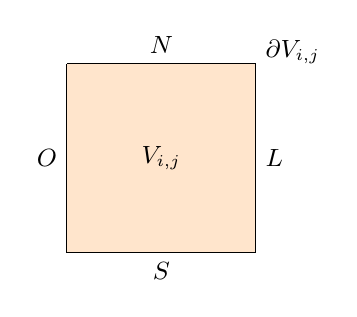
\begin{tikzpicture}[scale=1.5]
      \fill[fill=orange!20] (-0.8,-0.8) rectangle (0.8,0.8);

      \draw[black] (-0.8,-0.8) -- (-0.8, 0.8);
      \draw[black] (-0.8,-0.8) -- ( 0.8,-0.8);
      \draw[black] ( 0.8, 0.8) -- ( 0.8,-0.8);
      \draw[black] ( 0.8, 0.8) -- (-0.8, 0.8);
      
      \node[font=\small] at (0,0) {$V_{i,j}$};

      \node[above, font=\small] at (0, 0.8) {$N$};
      \node[below, font=\small] at (0,-0.8) {$S$};
      \node[right, font=\small] at ( 0.8,0) {$L$};
      \node[left,  font=\small] at (-0.8,0) {$O$};
      
      \node[right, font=\small] at (.8,.9) {$\partial V_{i,j}$};

  \end{tikzpicture}
  \caption{Componentes norte, sul, leste e oeste em $\partial V_{i,j}$.}
  \label{nsloEmPartialV}
  \end{figure}
\end{frame}

%----------------------------------------------------------------------------------------

\begin{frame}{Caso bidimensional}
  Com isso, têm-se
  \begin{equation}\label{integracaoDasFaces}
    \int_{\partial V_{i,j}}u \cdot n\ ds = \int_{N}u \cdot n_N\ ds + \int_{S}u \cdot n_S\ ds + \int_{L}u \cdot n_L\ ds + \int_{O}u \cdot n_O\ ds,
  \end{equation}
  em que $n_N$, $n_S$, $n_L$ e $n_O$ são os vetores normais a cada aresta de $\partial V_{i,j}$, apontando para fora do volume. Usando a discretização conservativa, pode-se aproximar cada integral separadamente, como por exemplo:
  \begin{align}
    \int_{S}u \cdot n_S\ ds &= \int_{x_{i-1/2}}^{x_{i+1/2}} K\left.\frac{\partial p}{\partial y}\right|_{(x,y_{j-1/2})}\ dx \\
    &\simeq \int_{x_{i-1/2}}^{x_{i+1/2}} -\frac{2K_{i,j-1}K_{i,j}}{K_{i,j-1}K_{i,j}}\left(\frac{p_{i,j} - p_{i,j-1}}{\Delta y}\right)\ dx \\
    &= \frac{\Delta x}{\Delta y} K_{i,j-\frac{1}{2}}(p_{i,j-1} - p_{i,j}),
  \end{align} 
  com $n_S = (0,-1)$, e similarmente para as outras faces.
\end{frame}

%----------------------------------------------------------------------------------------

\begin{frame}{Caso bidimensional}
  Portanto, a forma discreta de \eqref{eq:eq44}\ para um problema bidimensional é
  \begin{equation}\label{eq436}
    \begin{aligned}
    q_{i,j} = &- \frac{1}{\Delta y^2} K_{i,j+\frac{1}{2}}p_{i,j+1} - \frac{1}{\Delta y^2} K_{i,j-\frac{1}{2}}p_{i,j-1} \\
    &- \frac{1}{\Delta x^2} K_{i+\frac{1}{2},j}p_{i+1,j} - \frac{1}{\Delta x^2} K_{i-\frac{1}{2},j}p_{i-1,j} \\
    &+ \left(\frac{1}{\Delta y^2} K_{i,j+\frac{1}{2}} + \frac{1}{\Delta y^2} K_{i,j-\frac{1}{2}} + \frac{1}{\Delta x^2} K_{i+\frac{1}{2},j} + \frac{1}{\Delta x^2} K_{i-\frac{1}{2},j}\right)p_{i,j},
    \end{aligned}
  \end{equation}
  onde se usam as médias harmônicas em$K_{i,j\pm 1/2}$ $K_{i\pm 1/2,j}$.
\end{frame}

%----------------------------------------------------------------------------------------

\begin{frame}{Caso bidimensional}
  Após a pressão ser calculada, o campo de velocidades pode ser calculado usando a mesma estratégia de aproximação dos fluxos nas integrais em $\partial V_{i,j}$. Pela definição da velocidade de Darcy \eqref{leiDeDarcy}:
    \[
      \mathsf{u} = 
      \begin{bmatrix}
        u \\ v
      \end{bmatrix} =
      \begin{bmatrix}
        -K\partial_xp \\ -K \partial_yp
      \end{bmatrix}.
    \]
    Usando-se da discretização dos fluxos discutida anteriormente, mantendo-se a aproximação conservativa de volumes finitos, consegue-se:
    \begin{equation*}
      \begin{aligned}
        u_L \simeq -K_{i+\frac{1}{2},j}\frac{p_{i+1,j} - p_{i,j}}{\Delta x}, && u_O \simeq -K_{i-\frac{1}{2},j}\frac{p_{i,j} - p_{i-1,j}}{\Delta x} \\
        v_N \simeq -K_{i,j+\frac{1}{2}}\frac{p_{i,j+1} - p_{i,j}}{\Delta y}, && v_S \simeq -K_{i,j-\frac{1}{2}}\frac{p_{i,j} - p_{i,j-1}}{\Delta y}.
      \end{aligned}
    \end{equation*}
    Para fins de visualização, o campo vetorial pode ser calculado no centro das células, fornecendo um campo discreto mais conveniente para a maioria das situações. Isso pode ser calculado por médias simples, da forma
    \begin{equation}
      \begin{aligned}
        u_{i,j} = \frac{u_L + u_O}{2} && \text{e} && v_{i,j} = \frac{v_N + v_S}{2}.
      \end{aligned}
    \end{equation}
\end{frame}

%----------------------------------------------------------------------------------------

\begin{frame}{Caso bidimensional: Implementação}
  Em contornos de tipo \textbf{Neumann}, há a imposição de um fluxo na fronteira:
  \[
    \begin{aligned}
      -K\frac{\partial p}{\partial n} = -(K\nabla p) \cdot n = g(x,y) && \text{em $\zeta \subset \partial V_{i,j}$,}
    \end{aligned}
  \]
  onde $g$ é uma função conhecida. Se $g$ é nula, têm-se um contorno do tipo \textbf{homogênea} e tomando o exemplo da face leste:
  \[
    \int_{L}(K\nabla p) \cdot n_L\ ds = 0.
  \]
  Portanto, sua contribuição na equação \eqref{integracaoDasFaces}\ será eliminada. Caso $g$ não seja nula, têm-se uma condição de contorno do tipo \textbf{não homogênea}:
  \[
    \int_{L}(K\nabla p) \cdot n_L\ ds = \int_{y_{j-1/2}}^{y_{j+1/2}}(K\nabla p) \cdot n_L\ dy = -\int_{y_{j-1/2}}^{y_{j+1/2}}g(x_{\frac{1}{2}},y)\ dy.
  \]
\end{frame}

%----------------------------------------------------------------------------------------

\begin{frame}{Caso bidimensional: Implementação}
  Desse modo, seria preciso integrar numericamente $g$, por exemplo, pela regra do trapézio:
  \[
    G_j = \int_{y_{j-1/2}}^{y_{j+1/2}}g(x_{\frac{1}{2}},y)\ dy \simeq \frac{\Delta y}{2}\left(g(x_{\frac{1}{2}},y_{i-\frac{1}{2}}) + g(x_{\frac{1}{2}},y_{i+\frac{1}{2}})\right),
  \]
  da forma que a equação \eqref{eq436}\ será modificada (no exemplo de quando $i = M$) para
  \[
    \begin{aligned}
    q_{M,j}  - \frac{G_j}{\Delta x \Delta y} =
    &- \frac{1}{\Delta y^2} K_{M,j+\frac{1}{2}}p_{M,j+1} - \frac{1}{\Delta y^2} K_{M,j-\frac{1}{2}}p_{M,j-1} - \frac{1}{\Delta x^2} K_{M-\frac{1}{2},j}p_{M-1,j} \\
    &+ \left(\frac{1}{\Delta y^2} K_{M,j+\frac{1}{2}} + \frac{1}{\Delta y^2} K_{M,j-\frac{1}{2}} + \frac{1}{\Delta x^2} K_{M-\frac{1}{2},j}\right)p_{M,j}.
    \end{aligned}
  \]
\end{frame}

%----------------------------------------------------------------------------------------

\begin{frame}{Caso bidimensional: Implementação}
  Em contornos de tipo \textbf{Dirichlet}, impõe-se uma pressão em alguma fronteira:
  \[
    \begin{aligned}
    p = g(x,y) && \text{em $\zeta \subset \partial V_{i,j}$,}
    \end{aligned}
  \]
  onde $g$ é uma função. Por exemplo, a face sul do volume $V_{i,1}$ está em $\zeta$, então a contribuição da integral deve ser recalculada para:
  \[
    \begin{aligned}
        \int_{S}(K\nabla p)\cdot n_S\ ds 
        &= \int_{x_{i-1/2}}^{x_{i+1/2}}-K\frac{\partial p}{\partial y}(x,y_{\frac{1}{2}})\ dx \\
        &\simeq \int_{x_{i-1/2}}^{x_{i+1/2}}-K\left(\frac{p_{i,1} - g\left(x,y_{\frac{1}{2}}\right)}{y_1 - y_{\frac{1}{2}}}\right)\ dx \\
        &= -2\frac{\Delta x}{\Delta y}K_{i,\frac{1}{2}}p_{i,1} + \frac{2}{\Delta y}K_{i,\frac{1}{2}}\int_{x_{i-1/2}}^{x_{i+1/2}}g(x,y_{\frac{1}{2}})\ dx.
    \end{aligned}
  \]
\end{frame}

%----------------------------------------------------------------------------------------

\begin{frame}{Caso bidimensional: Implementação}
  E novamente, integra-se $g$ em $G_i$:
  \[
    G_i = \int_{x_{j-1/2}}^{x_{j+1/2}}g(x,y_{\frac{1}{2}})\ dx \simeq \frac{\Delta x}{2}\left(g(x_{i-\frac{1}{2}},y_{\frac{1}{2}}) + g(x_{i+\frac{1}{2}},y_{\frac{1}{2}})\right),
  \]
  e portanto, a equação \eqref{eq436}\ será modificada (no exemplo de quando $j = 1$) para 
  \[
    \begin{aligned}
    q_{M,j}  - \frac{2}{\Delta y^2 \Delta x}G_iK_{i,\frac{1}{2}} =
    &- \frac{1}{\Delta y^2} K_{i,\frac{3}{2}}p_{i,2} - \frac{1}{\Delta x^2} K_{i+\frac{1}{2},1}p_{i+1,1} - \frac{1}{\Delta x^2} K_{i-\frac{1}{2},1}p_{i-1,j} \\
    &+ \left(\frac{1}{\Delta y^2} K_{i,\frac{3}{2}} + \frac{2}{\Delta y^2} K_{i,\frac{1}{2}} + \frac{1}{\Delta x^2} K_{i+\frac{1}{2},1} + \frac{1}{\Delta x^2} K_{i-\frac{1}{2},1}\right)p_{i,1},
    \end{aligned}
  \]
  com $K_{i,\frac{1}{2}} = K_{i,1}$. Da mesma forma como no contorno de Neumann, quando $g \neq 0$, a condição de contorno de Dirichlet é do tipo \textbf{não homogêneo} e, caso contrário, \textbf{homogêneo}.
\end{frame}

%----------------------------------------------------------------------------------------

\begin{frame}{Caso bidimensional: Implementação}
  Considerando uma discretização $M \times N$ células computacionais, o esquema \eqref{eq436} pode ser escrito na forma matricial
  \[
    Aw = d
  \]
  com $w = (p_1,...,p_{MN})^t$ e $b = (q_1,...,q_{MN})^t$. Cada linha da matriz $A$ está relacionada com uma célula $(i,j)$ e leva em consideração as contribuições de seus quatro vizinhos. Para ordenar as células no caso bidimensional, pode-se escolher (dentre as triviais) ordenar \textit{por colunas} ou \textit{por linhas}; por exemplo, em uma malha $3 \times 3$, as células podem ser ordenadas (por linhas) da esquerda para direita, de cima para baixo, como a figura \ref{fig:ord_comp}.

  \begin{figure}[H]
  \centering
  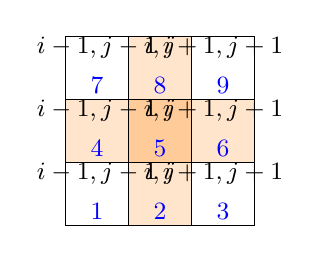
\begin{tikzpicture}[scale=1]
    \fill[fill=orange!20] (-0.4,1.2) rectangle (0.4,-1.2);
    \fill[fill=orange!20] (-1.2,0.4) rectangle (1.2,-0.4);
    \fill[fill=orange!40] (-0.4,0.4) rectangle (0.4,-0.4);

    \draw[black] (-1.2,-1.2) rectangle (1.2,1.2); % Desenha o quadrado

    % Linhas verticais (dividindo em 3 colunas)
    \draw[black] (-0.4,-1.2) -- (-0.4,1.2); % 1ª linha vertical
    \draw[black] ( 0.4,-1.2) -- ( 0.4,1.2);   % 2ª linha vertical

    % Linhas horizontais (dividindo em 3 linhas)
    \draw[black] (-1.2,-0.4) -- (1.2,-0.4); % 1ª linha horizontal
    \draw[black] (-1.2,0.4) -- (1.2,0.4);   % 2ª linha horizontal
    
    \node[below, font=\small, blue] at (-0.8,-0.8) {$1$};
    \node[below, font=\small, blue] at ( 0.0,-0.8) {$2$};
    \node[below, font=\small, blue] at ( 0.8,-0.8) {$3$};
    \node[below, font=\small, blue] at (-0.8, 0.0) {$4$};
    \node[below, font=\small, blue] at ( 0.0, 0.0) {$5$};
    \node[below, font=\small, blue] at ( 0.8, 0.0) {$6$};
    \node[below, font=\small, blue] at (-0.8, 0.8) {$7$};
    \node[below, font=\small, blue] at ( 0.0, 0.8) {$8$};
    \node[below, font=\small, blue] at ( 0.8, 0.8) {$9$};

    \node[above, font=\small, black] at (-0.8,-0.8) {$i-1,j-1$};
    \node[above, font=\small, black] at ( 0.0,-0.8) {$i  ,j  $};
    \node[above, font=\small, black] at ( 0.8,-0.8) {$i+1,j+1$};
    \node[above, font=\small, black] at (-0.8, 0.0) {$i-1,j-1$};
    \node[above, font=\small, black] at ( 0.0, 0.0) {$i  ,j  $};
    \node[above, font=\small, black] at ( 0.8, 0.0) {$i+1,j+1$};
    \node[above, font=\small, black] at (-0.8, 0.8) {$i-1,j-1$};
    \node[above, font=\small, black] at ( 0.0, 0.8) {$i  ,j  $};
    \node[above, font=\small, black] at ( 0.8, 0.8) {$i+1,j+1$};
  \end{tikzpicture}
  \caption{Exemplo de ordenação das células computacionais para um problema bidimensional.}
  \label{fig:ord_comp}
  \end{figure}
\end{frame}

%----------------------------------------------------------------------------------------

\begin{frame}{Caso bidimensional: Implementação}

\end{frame}

%----------------------------------------------------------------------------------------



%----------------------------------------------------------------------------------------



%----------------------------------------------------------------------------------------



%----------------------------------------------------------------------------------------